% LTeX: language=it
\documentclass[a4paper, 11pt, Arial]{article}

%\usepackage{mathrsfs}
\usepackage{amssymb}
\usepackage{amsmath}
\usepackage{array}
\usepackage{epsfig}
\usepackage{float}
\usepackage[margin=2cm]{geometry}
%\usepackage[sectionbib]{chapterbib}
\usepackage{fancyhdr}
\usepackage{lastpage}
\usepackage{graphicx}
\usepackage{caption}
\usepackage{subcaption}
\usepackage{array}
\usepackage{amsfonts}
%\usepackage{color}
\usepackage[usenames,dvipsnames]{color}
\usepackage[hyperindex, linktocpage]{hyperref}
\usepackage[italian]{babel}
\usepackage{wrapfig}
% \renewcommand{\rmdefault}{phv} % Arial
% \renewcommand{\sfdefault}{phv} % Arial

%%%%%%%%%%%%%%%%%%%%%%%%%%%%%%
\newcommand{\class}{Laboratorio di Automatica}
\newcommand{\expT}{Anti-windup e Feedforward}
\newcommand{\repN}{2}
\newcommand{\stud}{Lorenzo Franceschetti, 2000263 | Leonardo Luigi Pepe, 2009734 | 
 Federico Saporiti, 2000264}
\newcommand{\dateD}{1 luglio 2023}

% \renewcommand{\textheight}{710pt}
% \renewcommand{\topmargin}{-12pt}

% !TODO:
% - Schema AW e FF
% - Controllare i grafici
% - Solo la parte sperimentale
% - Max 5 pagine
% - Conclusioni

% Anti-windup e feed-forward
% 

\begin{document}

%\renewcommand{\baselinestretch}{1.5}

\begin{center}
\begin{tabular}{| p{\textwidth} |}
    \hline
    \large
    \vspace{-2pt}
    \stud \hfill
    \Large
    \begin{center}
    {\color{BrickRed}
        \textsl{\class}\\
        \textsl{Relazione n.\repN: \expT}\\
        \large
        \dateD}
    \vspace{-4mm}
    \end{center}\\
    \hline
\end{tabular}
\end{center}

\section{Introduzione}
\subsection{Scopo dell'attività}
Per migliorare le caratteristiche di un controllore PI di velocità di un motore in corrente continua, si può ricorrere ad alcune tecniche. In particolare, quelle implementate e analizzate in questa relazione sono l'anti-windup e il feedforward. Grazie a questi due schemi, è possibile migliorare la velocità di risposta del sistema retroazionato.

\subsection{Organizzazione della relazione}
L'elaborato si scompone in due parti. Nella prima parte si progetta e analizza uno schema anti-windup che permette di mitigare il problema della saturazione, dovuta al convertitore analogico digitale, confrontando i risultati con un modello privo di questa soluzione; nella seconda parte si aggiunge al controllore così ottenuto un compensatore feedforward, che rende il sistema più reattivo nell'inseguire il segnale di riferimento, riducendo il tempo di assestamento.

\subsection{Modello di partenza}
Di seguito è riportato il modello sperimentale del sistema di controllo di partenza
\begin{figure}[H]
    \centering
    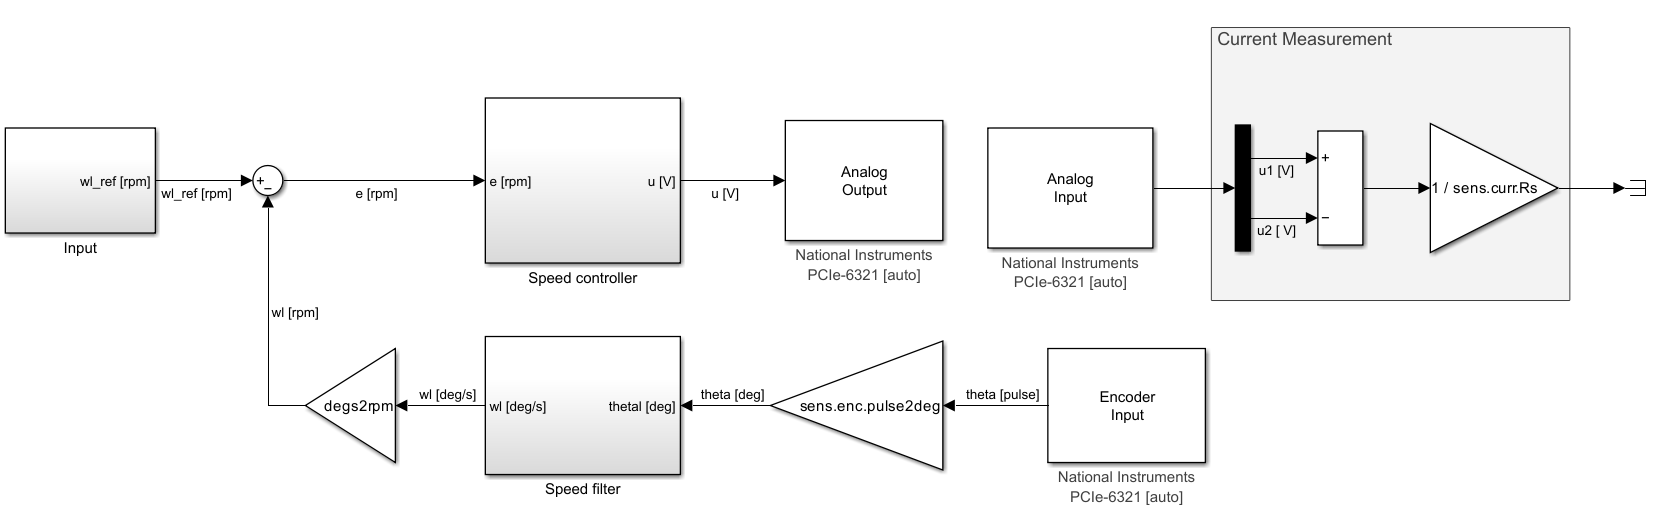
\includegraphics[width=\linewidth]{Images/original.png}
    \caption{Schema originale del sistema di controllo}
    \label{sim:initial}
\end{figure}
Il controllore di velocità è un controllore PI, che permette di avere un inseguimento a regime di un segnale costante con errore nullo. I coefficienti scelti sono $K_{P} = 0.0298$ e $K_{I} = 6.5015$, che permettono di avere un tempo di assestamento al 5\% pari a $t_{s, 5\%} = 0.145s$. Per misurare la velocità si è ricorsi a un filtro del secondo ordine a tempo continuo, nella forma
\begin{equation}
    H_{speed}(s) = \frac{\omega_{c}^2 s}{s^2 + 2 \delta \omega_{c} s + \omega_{c}^2}
    \label{sim:speed_filter}
\end{equation}
con $\omega_{c} = 2 \pi 50$ e $\delta = \frac{1}{\sqrt{2}}$.

\section{Anti-windup}
\iffalse
- Saturazione nel sistema reale
- Caricamento dell'azione integrale per portare l'attuatore fuori dalla saturazione

- Descrizione del windup
- Elementi che danno saturazione
- Schema anti-windup
- Confronto risultati sperimentali
- Conclusioni
\fi
\subsection{Descrizione}
Usando un controllore con azione integrale, può verificarsi un fenomeno chiamato windup. Questo avviene quando il segnale di errore $e$ è tale che il segnale di controllo $u_{c}$ generato dal controllore porta l'attuatore in saturazione. Il controllore continua ad integrare $e$, incrementando quindi $u_{c}$, senza che questo abbia una reale conseguenza sul processo. Quando $e$ diventa nullo, l'attuatore è ancora in saturazione, dato che l'integratore ha accumulato un grande errore di inseguimento nella fase iniziale. Per poter tornare nella regione di funzionamento lineare, $e$ deve assumere un valore negativo per un certo periodo di tempo, allontanandosi dal riferimento dato e dando origine a un importante fenomeno di sovraelongazione.

\subsection{Analisi della saturazione nel modello}
Nel sistema in analisi ci sono due elementi che possono dare origine a saturazione. Il primo è il convertitore digitale-analogico (DAC), che converte il segnale di controllo in uscita dal controllore alla tensione corrispondente. Questo elemento può produrre una tensione tra $-V_{sat_{DAC}}$ e $V_{sat_{DAC}}$, con $V_{sat_{DAC}} = 10V$. L'altro elemento è il driver di tensione, che va in saturazione per tensioni in uscita maggiori in modulo di $V_{sat_{DRV}} = 12V$. Questo componente ha un guadagno di tensione pari a $k_{drv} = 0.6V$ e il suo ingresso è collegato all'uscita del DAC. Dunque, se il DAC è in saturazione, l'uscita del driver è pari a $V_{max} = k_{drv} V_{sat_{DAC}} = 6V$, al di sotto della soglia di saturazione dello stesso. L'unico elemento di cui bisogna tenere conto è quindi il DAC.

\subsection{Schema anti-windup}
\begin{figure}[H]
    \centering
    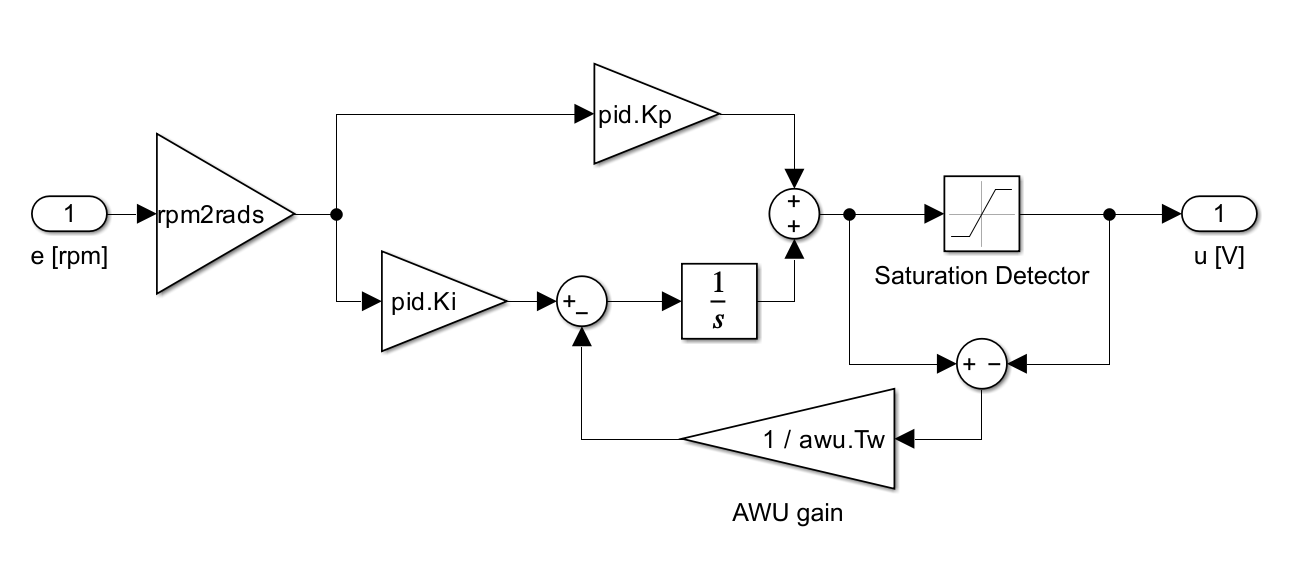
\includegraphics[width=0.7\linewidth]{Images/awu.png}
    \caption{Schema del sistema anti-windup}
    \label{sim:awu}
\end{figure}
Per mitigare questo fenomeno, si è modificato il controllore PI, aggiungendo un sistema di rilevazione e correzione del windup (figura \ref{sim:awu}). Il blocco Simulink di saturazione è impostato in modo che la regione lineare si trovi tra $-V_{sat_{DAC}}$ e $V_{sat_{DAC}}$, in modo da inviare al DAC un segnale nei suoi limiti di saturazione. Se la differenza tra il segnale di ingresso e quello di uscita non è nulla, è presente saturazione. Per correggerla, si compensa l'ingresso della componente integrale con un segnale proporzionale al valore di saturazione presente. Il guadagno è stato scelto pari a $K_{w} = 1 / T_{w}$, dove abbiamo scelto di usare $T_{w} = 0.03s \approx t_{s, 5\%} / 5$. Questo valore non è però necessariamente il migliore possibile per questa applicazione. Si rende quindi necessario effettuare più esperimenti, in modo da tararlo più finemente.

\subsection{Risultati sperimentali}
In laboratorio si è confrontata la risposta al gradino del sistema, prima disabilitando l'anti-windup e poi abilitandolo. Si riportano di seguito i dati ottenuti con un segnale a gradino di ampiezza $450rpm$ che agisce a $t_{0} = 1s$.
\begin{figure}[H]
    \centering
    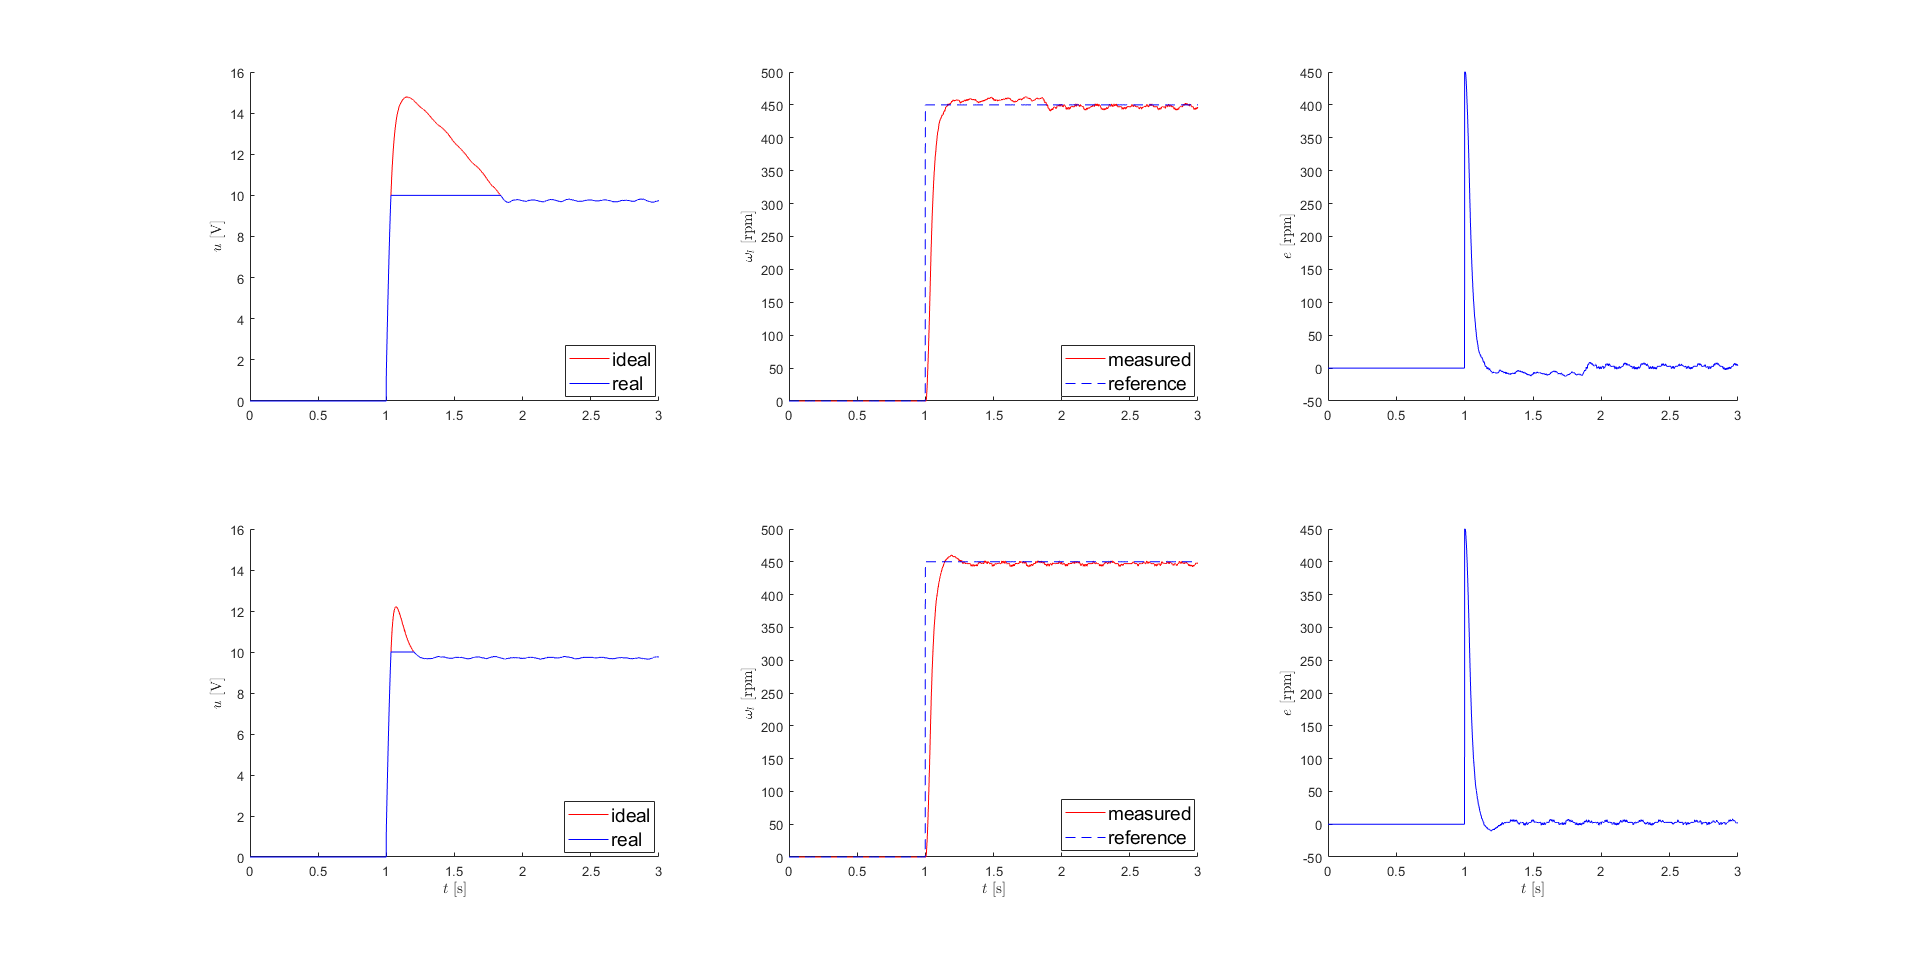
\includegraphics[width=\linewidth]{Images/awu_resp.png}
    \caption{Risposta al gradino}
    \label{awu:step}
\end{figure}
La prima riga si riferisce al controllore privo di anti-windup, mentre la seconda è riferita al sistema compreso di anti-windup.

\subsection{Conclusioni}
Dai risultati sperimentali ottenuti si può dedurre che il controllore dotato di uno schema anti-windup impiega meno tempo ad assestarsi sul riferimento costante, con una sovraelongazione minore rispetto all'altro. A questa conclusione si può giungere anche confrontando i grafici dell'ultima colonna della figura \ref{awu:step}, dove è rappresentato l'andamento dell'errore nel tempo. Nel caso del sistema privo di anti-windup, l'errore rimane per più tempo negativo, dovendo il sistema ritornare nella regione di funzionamento lineare dell'attuatore. Confrontando il valore delle tensioni di controllo nei due casi, è evidente come l'anti-windup porti a un picco minore di tensione richiesto e riduca notevolmente l'intervallo di tempo in cui il sistema si trova in saturazione. Lo schema anti-windup utilizzato migliora quindi le prestazioni del controllore.

\section{Feedforward}
\iffalse
- Descrizione del feedforward
- Schema feedforward
- Confronto risultati sperimentali
- Conclusioni
\fi
\subsection{Descrizione}
Uno schema di controllo in feedback permette di stabilizzare processi instabili e inseguire con errore nullo a regime il riferimento assegnato. Per migliorare la velocità di risposta è possibile ricorrere a uno schema feedforward, tramite il quale, pre-filtrando il segnale di riferimento, è possibile far variare istantaneamente l'uscita portandola al valore di riferimento e mantenendola poi tramite un controllo in feedback. Questo schema di controllo permette anche di eliminare il disturbo costante dovuto all'attrito del motore.

\subsection{Schema feedforward con anti-windup}
\begin{figure}[H]
    \centering
    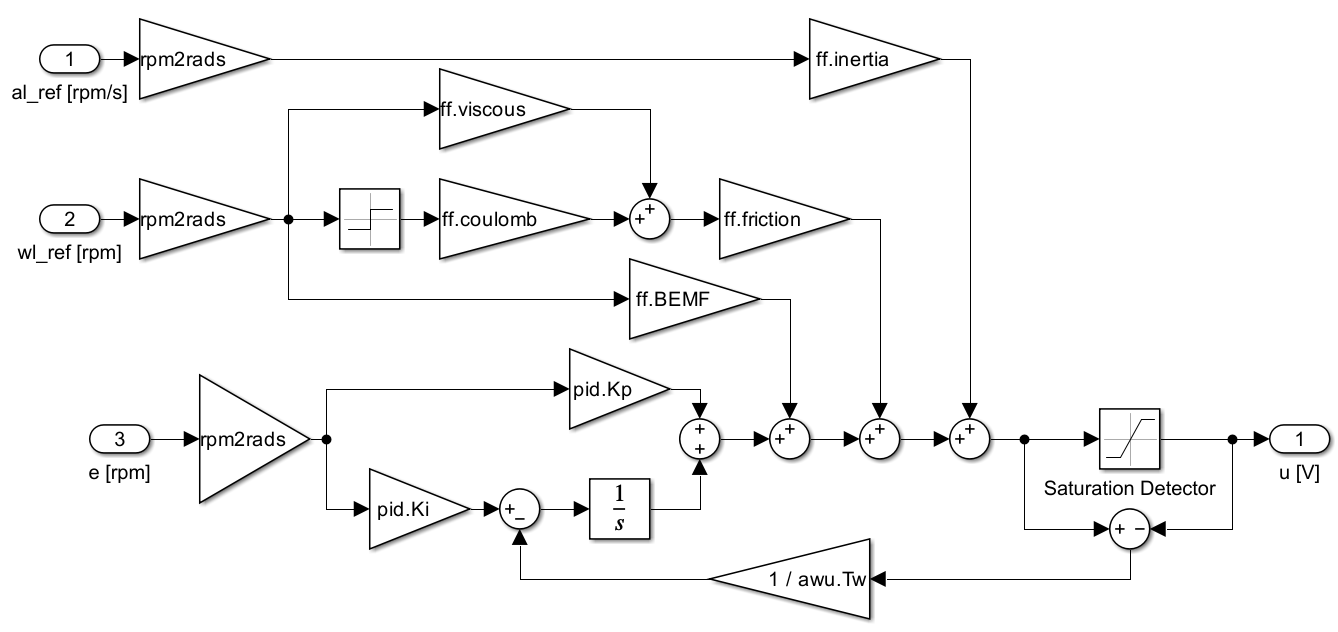
\includegraphics[width=0.7\linewidth]{Images/ff.png}
    \caption{Schema del controllore con feedforward e anti-windup}
    \label{sim:ff}
\end{figure}
Si è modellato il motore elettrico con una funzione di trasferimento del primo ordine $P(s)$ priva di zeri. L'azione compensatrice risulta essere descritta dalla funzione di trasferimento $H_{1}(s) = 1 / P(s) = \frac{N}{k_{m}}(T_{m} s + 1)$, non propria. Per poter dunque usare questo schema è necessario conoscere in anticipo la derivata del segnale di riferimento imposto. Per eliminare il disturbo dovuto all'attrito, si è riportata l'azione del momento di attrito all'ingresso del driver. In questo modo, la funzione di trasferimento per compensare questo disturbo risulta essere $H_{2}(s) = \frac{R_{eq}}{k_{drv} K_{t} N} \tau_{sf} sign(\omega_{l_{ref}})$. Chiamando $u_{1}$ l'azione compensatrice di $P(s)$ e $u_2$ l'azione compensatrice del momento di attrito, si ottiene che l'azione complessiva, applicata all'uscita del controllore prima dell'azione di anti-windup, è data da
\begin{equation}
    u_{ff} = u_{1} + u_{2} = \frac{N R_{eq} J_{eq}}{k_{drv} K_{t}} \frac{d\omega_{l_{ref}}}{dt} + 
                            \frac{R_{eq}}{k_{drv} K_{t} N} (N^2 B_{eq} \omega_{l_{ref}} + \tau_{sf} sign(\omega_{l_{ref}})) + \frac{N K_{e}}{k_{drv}} \omega_{l_{ref}}
  \label{ff:tf}
\end{equation}
con $\omega_{l_{ref}}$ riferimento di velocità al carico.

\subsection{Risultati sperimentali}
Per poter ottenere un risultato soddisfacente, è necessario che i valori usati siano quanto più vicini possibili a quelli reali. In particolare, è stato necessario stimare i valori di $B_{eq}$, $J_{eq}$ e $\tau_{sf}$, che sono risultati essere $\hat{B_{eq}} = 1.11221\cdot 10^{-6} \frac{Nm}{rad/s}$, $\hat{J_{eq}} = 5.7419 \cdot 10^{-7} kg\ m^2$ e $\hat{\tau_{sf}} = 9.6 \cdot 10^{-3} Nm$. Sono state effettuate due prove, disabilitando il feedforward nella prima e abilitandolo nella seconda. In entrambi i casi si è usato l'anti-windup, con $T_{w} = 0.03s$.

Si riportano di seguito i dati ricavati, utilizzando un riferimento di accelerazione costante a tratti definito in un periodo come
\begin{equation}
    a_{l_{ref}}(t) = 
    \begin{cases}
        900 rpm/s & \text{if 0 $\le$ $t$ $<$ 0.5s}\\
        0 & \text{if 0.5s $\le$ $t$ $<$ 1s}\\
        -900 rpm/s & \text{if 1s $\le$ $t$ $<$ 2s} \\
        0 & \text{if 2s $\le$ $t$ $<$ 2.5s}\\
        900 rpm/s & \text{if 2.5s $\le$ $t$ $<$ 3s}\\
    \end{cases}
\end{equation}

\begin{figure}[H]
    \centering
    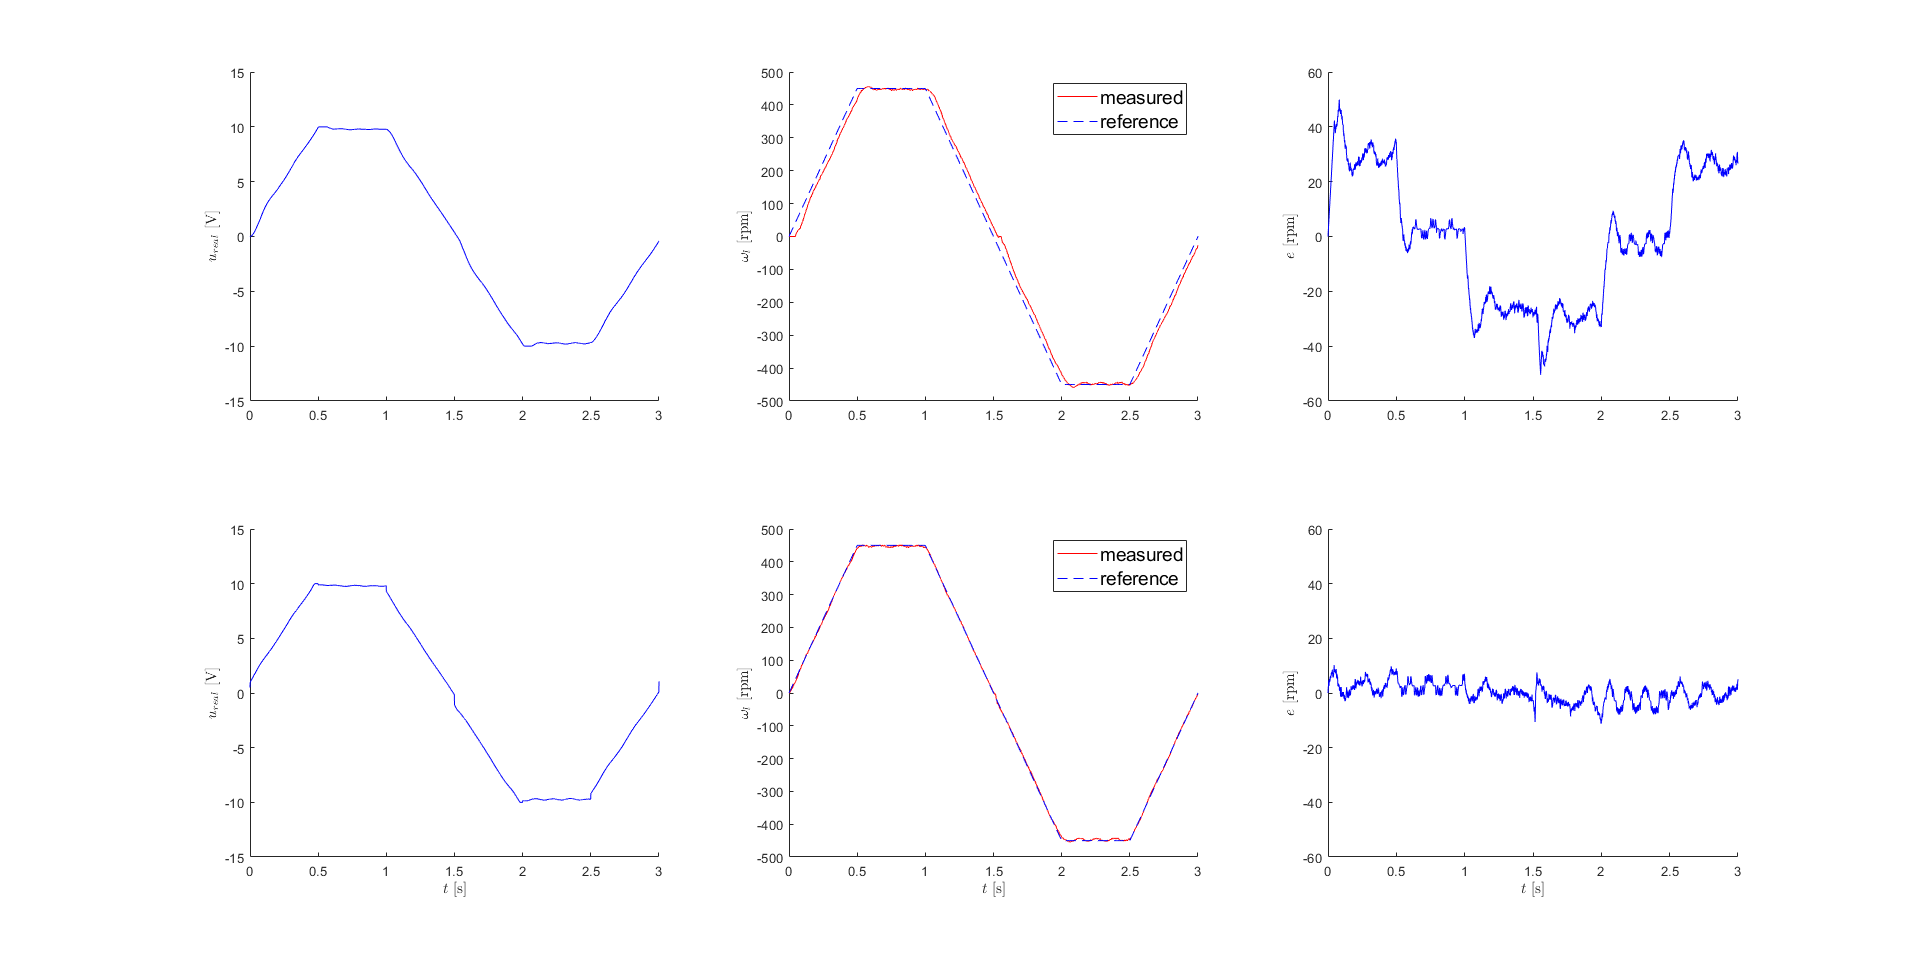
\includegraphics[width=\linewidth]{Images/ff_resp.png}
    \caption{Risposta al segnale}
    \label{ff:step}
\end{figure}
La prima riga si riferisce al controllore privo di feedforward, mentre la seconda è riferita al sistema compreso di feedforward.

\subsection{Conclusioni}
Nella seconda colonna della figura \ref{ff:step} sono riportate le velocità misurate nei due casi, confrontate con il riferimento dato. Si nota come l'azione di feedforward permetta al sistema di reagire in maniera più veloce alle variazioni di ingresso, aiutando il sistema a mantenersi vicino al riferimento anche per basse velocità. Al contrario, nel sistema privo di questo schema la velocità misurata presenta, nei tratti di accelerazione e decelerazione, un ritardo nell'assestamento. Come riportato nei grafici dell'ultima colonna, su cui è rappresentato l'errore rispetto al riferimento di velocità nei due casi, l'assenza del feedforward causa grandi variazioni nell'errore a seconda del tratto considerato, con picchi nei tratti in cui la velocità varia. Usandolo, invece, è possibile mantenere l'errore in una regione ridotta, senza grandi variazioni.

\section{Considerazioni finali}
Un controllore PI permette di inseguire un segnale costante con errore nullo a regime, ma, come si è potuto osservare nelle due esperienze qui descritte, presenta delle limitazioni dovute alle non idealità del processo da controllare, come la saturazione. In questo caso, un sistema di anti-windup permette di ridurre notevolmente il periodo di tempo necessario al controllore per assestarsi sul riferimento, riducendo anche la tensione di picco richiesta. Come si è visto successivamente, aggiungendo anche uno schema feedforward è possibile ridurre ulteriormente il tempo richiesto al sistema per raggiungere il riferimento, permettendo anche di ridurre l'errore rispetto ad esso. Il sistema implementato, però, richiede una perfetta conoscenza della derivata del segnale di riferimento, non sempre ottenibile. Una possibile modifica, per rendere lo schema compatibile con situazioni in cui la derivata non è nota a priori, è quella di calcolare la derivata del riferimento tramite un filtro del secondo ordine, con la stessa struttura del filtro $H(s)$ usato per misurare la velocità dall'angolo misurato.

\end{document}
